\documentclass{beamer}
\usetheme{metropolis}

\usepackage{tikz}
\usepackage{listings}
\usepackage{xcolor}
\usepackage{soul}
\usepackage{colortbl}

\usepackage[french]{babel}

% Set graphics folder path
\graphicspath{{./images/}}

\usetikzlibrary{automata,arrows}


%% Listing properties

% C listings
\lstset{
  language=C,
  escapeinside={@}{@},
  showstringspaces=false,
  keywordstyle=\itshape\color{blue},
  xleftmargin=0pt,
  xrightmargin=0pt,
}

% JSON listings
\colorlet{punct}{red!60!black}
\definecolor{delim}{RGB}{20,105,176}

\lstdefinelanguage{json}{
    literate=
      *{:}{{{\color{punct}{:}}}}{1}
      {,}{{{\color{punct}{,}}}}{1}
      {\{}{{{\color{delim}{\{}}}}{1}
      {\}}{{{\color{delim}{\}}}}}{1}
      {[}{{{\color{delim}{[}}}}{1}
      {]}{{{\color{delim}{]}}}}{1},
}

%% Define color for code highlight
\definecolor{light-gray}{gray}{0.80}

%% Tikz commands

%% Define a tikz marks to print user defined tikz graphics at specific
%% position on the slide
\usetikzlibrary{positioning,decorations.pathreplacing,fit}
\newcommand{\tikzmark}[2][]{%
  \tikz[remember picture,overlay,baseline=-.5ex] \node[#1] (#2) {};%
}

%% Draw brace between two tikzmarks

% \drawBrace[xshift]{beginningNode}{endingNode}
% This command draws a brace between two tikzmarks, to their right,
% no matter which one is the rightmost, and includes
% a node midway the brace, to write the comment.
% This command also creates a new node
% whose name is the concat of the names of beginning and ending nodes.
%
% Example :
% \begin{lstlisting}[name=listing,escapechar=!]
%   Example code line 1 !\tikzmark{bgnShifted}!
%   Example code line 2
%   Example code line 3
%   Example code line 4 !\tikzmark{bgnBrace}\tikzmark{trmShifted}!
%   Example code line 5
%   Example code line 6
%   Example code line 7 !\tikzmark{trmBrace}!
%   Example code line 8
%   Example code line 9 !\tikzmark{bgnOther}!
%   Example code line 10 !\tikzmark{trmOther}!
% \end{lstlisting}

% \begin{tikzpicture}[overlay, remember picture]
%     \drawBrace[.6em]{bgnShifted}{trmShifted}{Example xshifted.};
%     \drawBrace{bgnBrace}{trmBrace}{Example annotation.};
%     \drawBrace{bgnOther}{trmOther}{Another example.};
% \end{tikzpicture}

\newcommand*{\drawBrace}[4][0pt]{%
    \node[draw=none, fit={(#2) (#3)}, inner sep=0pt] (rectg) {};%
    \draw [decoration={brace,amplitude=0.3em},decorate,very thick,red]%
      ([xshift=#1]rectg.north east) --%
      coordinate[right=1em, midway] (#2#3)
      ([xshift=#1]rectg.south east);%
    \node[right=1.5em of #2#3] (#2#3-comment) {#4};
    \draw (#2#3-comment.west) edge (#2#3);
}%

%% Draw an horizontal arrow from a tikzmark,
%% with a comment at the end

\newcommand{\drawArrow}[3][1.5em]{%
  \node[right=#1 of #2] (#2-comment) {#3};
  \draw[->, red, thick] (#2) -- (#2-comment);
}%

% Place a Latex command at a specified position
% Usage:
% \tikzoverlay at (-1cm,-5cm) {content};
% or
% \tikzoverlay[text width=5cm] at (-1cm,-5cm) {content};
\def\tikzoverlay{%
   \tikz[baseline,overlay]\node[anchor=north west]
}%

% \title{Étendre LTL par des positions du code et des variables locales}
\title{Surmonter les limites des assertions et de LTL}

\date{2018-01-25}
\author{Guillaume \bsc{Hétier}}
\institute{Polytechnique Montréal}

\begin{document}
\maketitle

% \section{Vérification formelle : le model checking}

%% Dire rapidement à l'oral les problèmes de sécu, les faiblesses du tests, etc.
%% Présentater LTL
%% Pas la peine de présenter les assertions
%% Présenter le concept du model checking + situer dans quelle étape du
%% processus on va se situer
%% Garder les exemples (mais bien les préparer)

\begin{frame}{Un grand risque d'erreurs}

  \tikzoverlay at (0cm, 1cm) {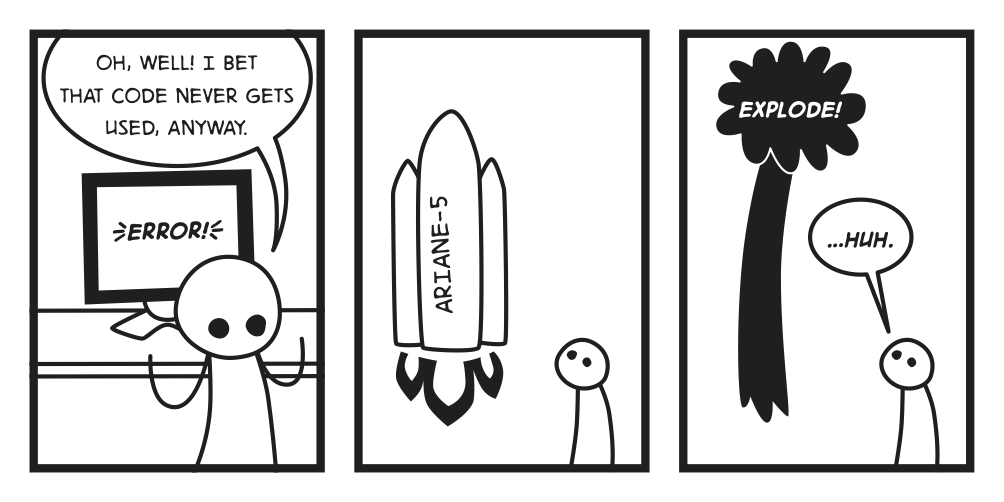
\includegraphics[width=0.8\textwidth]{ariane-rocket-cartoon.png}};
  \tikzoverlay at (2cm, 4cm) {
\includegraphics[width=0.3\textwidth]{spectre_meltdown.png}};
  \tikzoverlay[label={below:Wannacry}] at (7.5cm, 4cm) {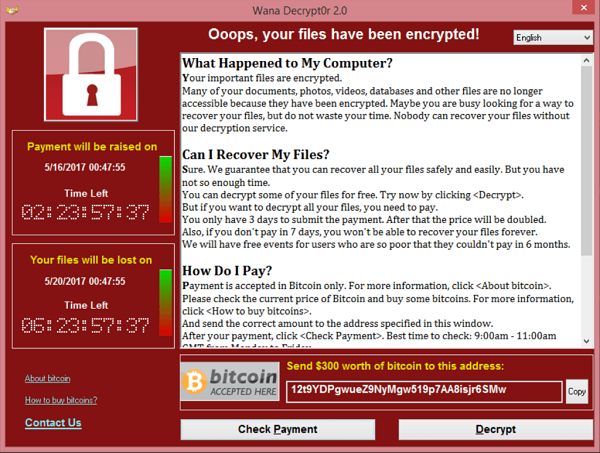
\includegraphics[width=0.3\textwidth]{wannacry.png}};

\end{frame}

\begin{frame}{Un exemple : un pacemaker}
  \begin{center}
  \begin{tikzpicture}
  \node[label=below:Batterie 1] at (0, 0) (bat_1) {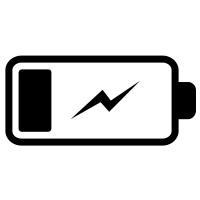
\includegraphics[width=0.1\textwidth]{battery.png}};
  \node[label=below:Batterie 2] at (4, 0) (bat_2) {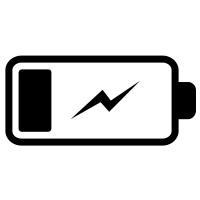
\includegraphics[width=0.1\textwidth]{battery.png}};

  \node at (2, 3) (pacemaker) {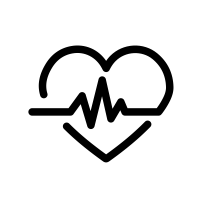
\includegraphics[width=0.1\textwidth]{hearth.png}};

  \draw[->] (bat_1) -- (pacemaker);
  \draw[->] (bat_2) -- (pacemaker);
  \end{tikzpicture}
  \end{center}

\end{frame}

\begin{frame}[fragile]{Un exemple}
\begin{columns}[onlytextwidth, T]
  \column{0.48\textwidth}
\begin{lstlisting}[caption=Thread 1, frame=single]
void* bat1(void* d) {
  int i, e = 100;
  for(i=0; i<3; i++) {
    while (e > 0)
        e--;
    // Recharge
    @\textcolor{red}{e = 100;}@
  }
  pthread_exit(NULL);
}
\end{lstlisting}

  \column{0.48\textwidth}
\begin{lstlisting}[frame=single, caption=Thread 2]
void* bat2(void* d) {
  int i, e = 100;
  for(i=0; i<3; i++) {
    while (e > 0)
        e--;
    // Recharge
    @\textcolor{red}{e = 100;}@
  }
  pthread_exit(NULL);
}
\end{lstlisting}
\end{columns}
\end{frame}

\begin{frame}[standout]
  Comment éviter de telles erreurs ?
\end{frame}


\begin{frame}{Le model-checking}

  \begin{tikzpicture}

  \node[label=below:\tiny Code] at (0, 0) (code_file) {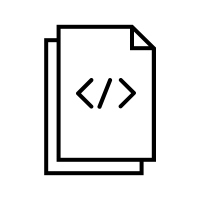
\includegraphics[width=0.1\textwidth]{code_file.png}};
  \node[label=below:\tiny Modèle] at (3, 0) (code_graph) {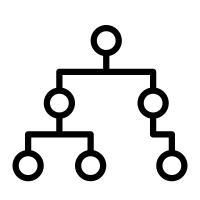
\includegraphics[width=0.1\textwidth]{graph.png}};

  \node[label={below:\tiny Spécification}] at (0, -3) (spec_file) {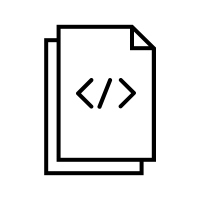
\includegraphics[width=0.1\textwidth]{code_file.png}};

  \node[label=right:\tiny Model checker] at (6, -1.5) (model_checker) {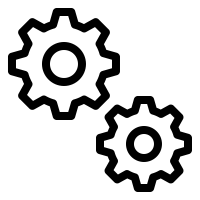
\includegraphics[width=0.1\textwidth]{gears.png}};

  \draw[->] (code_file) -- (code_graph);
  \draw[->] (code_graph) -- (model_checker);
  \draw[->] (spec_file) -- (model_checker);
\end{tikzpicture}
\end{frame}

\section{Limites des formalismes de spécification actuels}

\begin{frame}[fragile]{Spécification --- Assertions}
\begin{center}
\texttt{assert(b1 > 10);}
\end{center}
\end{frame}

\begin{frame}{Spécification --- Assertions}
  \begin{tikzpicture}
    \node at (0, -2) (assert_1) {\texttt{assert(b1>0 \&\& ???)}};
    \draw[->, blue, thick] (0,0) -- (assert_1);
    \draw[->, blue, thick] (assert_1) -- (0, -4);

    \node at (6, -2) (assert_2) {\texttt{assert(b2>0 \&\& ???)}};
    \draw[->, blue, thick] (6,0) -- (assert_2);
    \draw[->, blue, thick] (assert_2) -- (6, -4);
  \end{tikzpicture}

  \vspace{1em}
  \begin{center}
  Comment exprimer des relations entre assertions ?
  \end{center}
\end{frame}

\begin{frame}{Spécification --- LTL}
  \begin{tikzpicture}[->, >=stealth', shorten >=1pt,auto,node distance=1.5cm,
                main node/.style={circle,draw}]

      \node[main node, initial left, initial text={\hspace{2ex}p : }] (1) {p};
      \node (2) [right of=1] {...};
      \draw (1) -- (2);
  \end{tikzpicture}

  \vspace{1em}

  \begin{tikzpicture}[->, >=stealth', shorten >=1pt,auto,node distance=1.5cm,
                main node/.style={circle,draw}]

      \node[main node, initial left, initial text={X(p) : }] (X1) {q};
      \node[main node] (X2) [right of=X1] {\textcolor{red}{p}};
      \node (X3) [right of=X2] {...};
      \draw (X1) -- (X2);
      \draw (X2) -- (X3);
  \end{tikzpicture}

  \vspace{1em}

  \begin{tikzpicture}[->, >=stealth', shorten >=1pt,auto,node distance=1.5cm,
                main node/.style={circle,draw}]

      \node[main node, initial left, initial text={G(p) : }] (G1) {\textcolor{red}{p}};
      \node[main node] (G2) [right of=G1] {\textcolor{red}{p}};
      \node[main node] (G3) [right of=G2] {\textcolor{red}{p}};
      \node[main node] (G4) [right of=G3] {\textcolor{red}{p}};
      \node (G5) [right of=G4] {...};
      \draw (G1) -- (G2);
      \draw (G2) -- (G3);
      \draw (G3) -- (G4);
      \draw (G4) -- (G5);
  \end{tikzpicture}

  \vspace{1em}

  \begin{tikzpicture}[->, >=stealth', shorten >=1pt,auto,node distance=1.5cm,
                main node/.style={circle,draw}]

      \node[main node, initial left, initial text={F(p) : }] (F1) {q};
      \node[main node] (F2) [right of=F1] {q};
      \node[main node] (F3) [right of=F2] {q};
      \node[main node] (F4) [right of=F3] {\textcolor{red}{p}};
      \node (F5) [right of=F4] {...};
      \draw (F1) -- (F2);
      \draw (F2) -- (F3);
      \draw (F3) -- (F4);
      \draw (F4) -- (F5);
  \end{tikzpicture}

\end{frame}

\begin{frame}{Spécification --- LTL}
    \begin{center}
      $G(\textcolor{red}{p} \implies F (\textcolor{red}{q}
      \lor \textcolor{red}{r}))$
    \end{center}
  \begin{block}{Propositions atomiques}
    \begin{itemize}
      \item Expressions booléennes
      \item Pas de positions du code
      \item Pas de variables locales
    \end{itemize}
  \end{block}
    \begin{center}
      $G(\textcolor{red}{\{x == 2\}} \implies F
      (\textcolor{red}{\{y == x\}}
      \lor \textcolor{red}{\{z >= x\}}))$
    \end{center}
\end{frame}

\begin{frame}[standout]{Notre objectif}
  \begin{enumerate}
    \setlength{\itemsep}{2em}
  \item Étendre LTL
    \begin{itemize}
      \item variables locales
      \item positions du code source
    \end{itemize}
  \item Méthode de vérification
    \begin{itemize}
      \item réduction à la vérification d'assertions
      \item transformation sources à sources
    \end{itemize}
  \end{enumerate}
\end{frame}

\section{Étendre LTL}

%% N'insister que sur les zone de validité, garder le reste en
%% annexe
%% Parler des différences avec Divine
\begin{frame}{Quels sont les obstacles à surmonter ?}
    \begin{enumerate}
    \item Identifier les variables locales
    \item Manipuler les positions du code
    \item \alert<2>{Prolonger la définition des propositions atomiques}
    \end{enumerate}
\end{frame}

\begin{frame}[fragile]{Définition des propositions atomiques}
\begin{columns}[onlytextwidth, c]
  \column{0.50\textwidth}

  \begin{block}{Problème}
  \begin{itemize}
    \setlength{\itemsep}{1.5em}
    \item $G \{\texttt{bat1::e} > 0\}$
    \item Comment évaluer la p.a dans \texttt{main} ?
  \end{itemize}
  \end{block}

  \vspace{3em}
  \alert{Hors du contexte d'existence de \texttt{bat1::e}, la p.a n'est pas définie.}

  \column{0.45\textwidth}

\begin{lstlisting}[language=C]
void* bat1(void* d) {
  @\colorbox{light-gray}{int i, \textcolor{red}{e} = 100;}@
  @\colorbox{light-gray}{for (i=0; i<3; i++) \{}@
  @\colorbox{light-gray}{\hspace{2ex}while (\textcolor{red}{e} > 0)}@
  @\colorbox{light-gray}{\hspace{4ex}\textcolor{red}{e}-{}-;}@
  @\colorbox{light-gray}{\hspace{2ex}\textcolor{red}{e} = 100;}@
  @\colorbox{light-gray}{\}}@
}
int main() {
  bat1();
  return 0;
}
\end{lstlisting}
\end{columns}
\end{frame}

\begin{frame}[fragile]{Zone de validité}
\begin{columns}[onlytextwidth, c]
  \column{0.50\textwidth}

  \begin{block}{Proposition atomiques}
  \begin{itemize}
  \item Zone de validité $\rightarrow$
    \item Fonction d'évaluation
      \begin{itemize}
        \item $\texttt{bat1::e} > 0$
      \end{itemize}
    \item Valeur par défaut
      \begin{itemize}
        \item \emph{True}
      \end{itemize}
  \end{itemize}
  \end{block}

  \column{0.45\textwidth}

\begin{lstlisting}[language=C]
void* bat1(void* d) {
  @\colorbox{light-gray}{int i, \textcolor{red}{e} = 100;}@
  @\colorbox{light-gray}{for (i=0; i<3; i++) \{}@
  @\colorbox{light-gray}{\hspace{2ex}while (\textcolor{red}{e} > 0)}@
  @\colorbox{light-gray}{\hspace{4ex}\textcolor{red}{e}-{}-;}@
  @\colorbox{light-gray}{\hspace{2ex}\textcolor{red}{e} = 100;}@
  @\colorbox{light-gray}{\}}@
}
int main() {
  bat1();
  return 0;
}
\end{lstlisting}
\end{columns}
\end{frame}

\begin{frame}[fragile]{Zone de validité}
\begin{lstlisting}
void* bat1(void* d) {
begin: @\colorbox{light-gray}{int i, e = 100;}@ @\tikzmark{bracket1_begin}@
       @\colorbox{light-gray}{for (i=0; i<3; i++) \{}@
       @\colorbox{light-gray}{\hspace{2ex}while (e > 0)}@
       @\colorbox{light-gray}{\hspace{4ex}e-{}-;}@
       @\colorbox{light-gray}{\hspace{2ex}e = 100;}@
       @\colorbox{light-gray}{\}}@ @\tikzmark{bracket1_end}@
end:   ;
}
int main() { @\tikzmark{bracket2_begin}@
  bat1();
  return 0;
} @\tikzmark{bracket2_end}@
\end{lstlisting}

\begin{tikzpicture}[overlay, remember picture]
    \drawBrace[2.2em]{bracket1_begin}{bracket1_end}{Fonction d'évaluation : $e > 0$};
    \drawBrace[5.3em]{bracket2_begin}{bracket2_end}{Valeur par défaut : Vrai};
\end{tikzpicture}

\end{frame}

\begin{frame}[fragile]{Exemple de spécification}

  \begin{columns}[onlytextwidth, c]

    \column{0.6\textwidth}
  \begin{lstlisting}[language=json]
{
  "ltl": "G(p)",
  "pa": [
    {
      "name": "p",
      "default": true,
      "expr": "f_ev", @\tikzmark{arrow1_begin}@
      "span": ["begin", "end"],
      "params": ["bat1::e"]
    }
  ]
}
\end{lstlisting}

    \column{0.3\textwidth}
\begin{lstlisting}[frame=l]
@\tikzmark{arrow1_end}@int f_ev(int e) {
  return e>0;
}
\end{lstlisting}

  \end{columns}

\begin{tikzpicture}[overlay, remember picture]
  \draw[->, red, thick] (arrow1_begin) -- (arrow1_end);
\end{tikzpicture}
\end{frame}

%% Supprimer la slide, remarques à l'oral uniquement
% \begin{frame}{Autres intérêts des zones de validités}
%   \begin{exampleblock}{Autres intérêts des zones de validités}
%   \begin{itemize}
%     \item problème de définitions des p.a
%     \item manipulation des positions
%     \item intervalles supportés dans les p.a
%     \item exclure les initialisations, \dots
%   \end{itemize}
%   \end{exampleblock}
% \end{frame}

\begin{frame}[fragile]{Cas des batteries}
\begin{columns}[onlytextwidth, T]
  \column{0.48\textwidth}
\begin{lstlisting}[caption=Thread 1, frame=single]
void* bat1(void* d) {
  int i, e = 100;
  for(i=0; i<3; i++) {
    while (e > 0)
        e--;
    // Recharge
    b1: @\colorbox{light-gray}{e = 100;}@
    e1: ;
  }
  pthread_exit(NULL);
}
\end{lstlisting}

  \column{0.48\textwidth}
\begin{lstlisting}[frame=single, caption=Thread 2]
void* bat2(void* d) {
  int i, e = 100;
  for(i=0; i<3; i++) {
    while (e > 0)
        e--;
    // Recharge
    b2: @\colorbox{light-gray}{e = 100;}@
    e2: ;
  }
  pthread_exit(NULL);
}
\end{lstlisting}
\end{columns}
\end{frame}

\begin{frame}[fragile]{Spécification des batteries}
  \begin{columns}
    \column{0.6\textwidth}
\begin{lstlisting}[basicstyle=\small, language=json]
{
  "ltl": "G(!(t1 && t2))",
  "pa": [ {
      "name": "t1",
      "default": false,
      "expr": "reload", @\tikzmark{arrow2_begin}@
      "span": ["b1", "e1"],
      "params": []
    }, {
      "name": "t2",
      "default": false,
      "expr": "reload", @\tikzmark{arrow3_begin}@
      "span": ["b2", "e2"],
      "params": []
    } ]
}
\end{lstlisting}
    \column{0.3\textwidth}
\begin{lstlisting}[frame=l]
@\tikzmark{arrow2_end}@int reload() {
  return 1;
}
\end{lstlisting}

  \end{columns}

\begin{tikzpicture}[overlay, remember picture]
  \draw[->, red, thick] (arrow2_begin) -- (arrow2_end);
  \draw[->, red, thick] (arrow3_begin) -- (arrow2_end);
\end{tikzpicture}
\end{frame}

%% TODO: améliorer la slide (contenu + présentation)
\begin{frame}{Bilan partie 1}
  \begin{block}{Contributions}
    \begin{itemize}
    \item zones de validité
    \item variables locales et positions
    \item englobe LTL et les assertions
    \end{itemize}
  \end{block}

  \begin{alertblock}{Limitations}
    \begin{itemize}
    \item verbeux
    \item Divine : alternative plus instinctive,
    mais plus invasive, moins bon support des positions
    \end{itemize}
  \end{alertblock}

\end{frame}

\section{Ramener LTL à la vérification d'assertions}

\begin{frame}{Faible support de LTL}
  Parmi les model-checkers logiciels pour le C concurrent :
  \begin{itemize}
    \item 14 passés en revue
    \item 14 supportent les assertions
    \item 1 seul supporte LTL
  \end{itemize}
\end{frame}

\begin{frame}[standout]
  Comment vérifier des propriétés LTL ?

  \vspace{2em}
  \small (et notre spécification ?)
\end{frame}

\begin{frame}{Automates de Büchi}
  \begin{columns}[onlytextwidth, c]
    \column{0.6\textwidth}

    \begin{itemize}
      \setlength{\itemsep}{1.5em}
    \item Un automate de Büchi représente une propriété LTL.
    \item Méthode de construction : \textbf{LTL2BA} [Gastin, Ouddoux]
    \end{itemize}

    \column{0.4\textwidth}
    \begin{center}
    Automate pour $F (p || q)$
    \vspace{1em}

\begin{tikzpicture}[->, shorten >=1pt, >=stealth',auto,node distance=2cm,
                thick,main node/.style={circle,draw}]

  \node[main node, initial above, initial text = {}] (1) {1};
  \node[main node, accepting] (2) [below of=1] {2};

  \path
    (1) edge [loop right] node {} (1)
    (1) edge  node {$p || q$} (2)
    (2) edge [loop right] node {} (2);
\end{tikzpicture}
    \end{center}

  \end{columns}

\end{frame}

\begin{frame}{Vérification de propriétés LTL}

  \begin{tikzpicture}

  \node[label=below:\tiny Code] at (0, 0) (code_file) {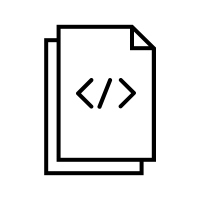
\includegraphics[width=0.1\textwidth]{code_file.png}};
  \node[label=below:\tiny Modèle] at (2, 0) (code_graph) {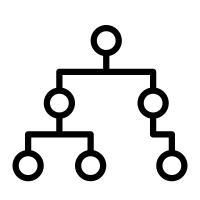
\includegraphics[width=0.1\textwidth]{graph.png}};

  \node[label={below:\tiny Spécification ($\Phi$)}] at (0, -2) (spec_file) {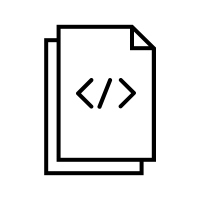
\includegraphics[width=0.1\textwidth]{code_file.png}};
  \node[label=below:\tiny Automate ($\lnot \Phi$)] at (2, -2) (spec_graph) {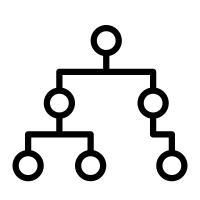
\includegraphics[width=0.1\textwidth]{graph.png}};

  \node[label=below:\tiny Produit] at (4, -1) (produit_graph) {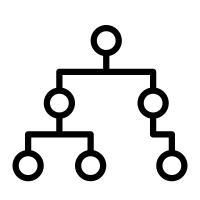
\includegraphics[width=0.1\textwidth]{graph.png}};

  \node[label=right:\tiny Exploration] at (7, -1) (model_checker) {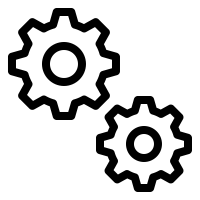
\includegraphics[width=0.1\textwidth]{gears.png}};

  \node[label={[green, font=\tiny\bf]below:Valide}] at (6, -3) (res_reject) {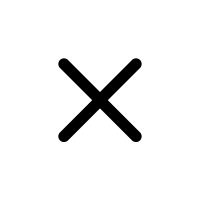
\includegraphics[width=0.1\textwidth]{reject.png}};
  \node[label={[align=center, red, font=\tiny\bf]below: Cycle acceptant :\\ Erreur + Contre-exemple}]
  at (8, -3) (res_accept) {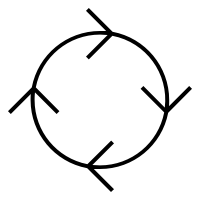
\includegraphics[width=0.1\textwidth]{cycle.png}};

  \draw[->] (code_file) -- (code_graph);
  \draw[->] (code_graph) -- (produit_graph);
  \draw[->] (spec_file) -- (spec_graph);
  \draw[->] (spec_graph) -- (produit_graph);
  \draw[->] (spec_graph) -- (produit_graph);
  \draw[->] (produit_graph) -- (model_checker);
  \draw[->] (model_checker) -- (res_accept);
  \draw[->] (model_checker) -- (res_reject);
\end{tikzpicture}

\end{frame}

\begin{frame}{Transformation source à source}

\begin{columns}[onlytextwidth, T]
  \column{0.45\textwidth}
  \begin{center}
    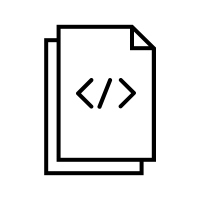
\includegraphics[width=0.5\textwidth]{code_file.png}\tikzmark{arrow1_begin}

  Code source d'origine + spécification

  \end{center}
  \column{0.45\textwidth}
  \begin{center}
  \tikzmark{arrow1_end}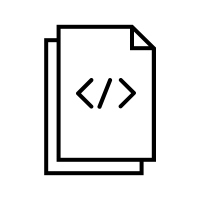
\includegraphics[width=0.5\textwidth]{code_file.png}

  Code source transformé + assertions
  \end{center}

\begin{tikzpicture}[overlay, remember picture]
  \draw[->, very thick, transform canvas={yshift=3em}](arrow1_begin) -- (arrow1_end);
\end{tikzpicture}

\end{columns}

\begin{block}{Invariant}
 Équivalence du respect de la spécification.
\end{block}

\end{frame}

\begin{frame}{Architecture de baProduct}

  \begin{tikzpicture}

  \node[label={below:\tiny Spécification ($\Phi$)}] at (0, -0.5) (spec_file) {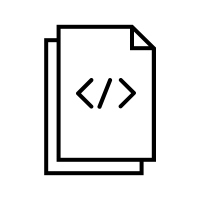
\includegraphics[width=0.1\textwidth]{code_file.png}};
  \node[label=below:\tiny Automate ($\lnot \Phi$)] at (2, -0.5) (spec_graph) {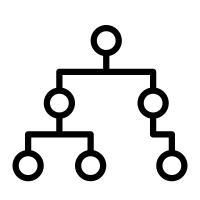
\includegraphics[width=0.1\textwidth]{graph.png}};
  \node[label={[align=left]right:\tiny Code de l'automate\\ \tiny(assertions)}] at (4, -0.5) (auto_file) {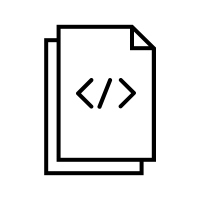
\includegraphics[width=0.1\textwidth]{code_file.png}};

  \node[label=below:\tiny Code] at (0, -3) (code_file) {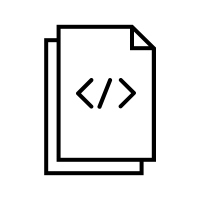
\includegraphics[width=0.1\textwidth]{code_file.png}};

  \node[label={below:\tiny Produit}] at (4, -3) (produit_file) {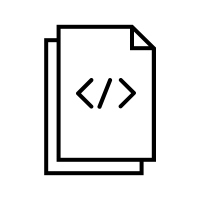
\includegraphics[width=0.1\textwidth]{code_file.png}};

  \node[label=right:\tiny Model-checker] at (7, -3) (model_checker) {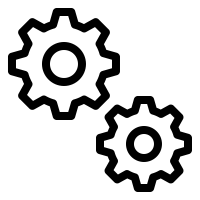
\includegraphics[width=0.1\textwidth]{gears.png}};

  \node[label={[green, font=\tiny\bf]below:Valide}] at (6, -5) (res_reject) {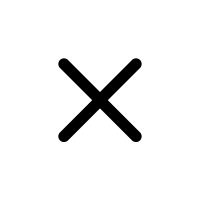
\includegraphics[width=0.1\textwidth]{reject.png}};
  \node[label={[red, font=\tiny\bf]below:Erreur}] at (8, -5) (res_accept) {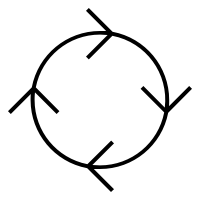
\includegraphics[width=0.1\textwidth]{cycle.png}};

  \draw[->] (code_file) -- (produit_file);
  \draw[->] (spec_file) -- (spec_graph);
  \draw[->] (spec_graph) -- (auto_file);
  \draw[->] (auto_file) -- (produit_file);
  \draw[->] (produit_file) -- (model_checker);
  \draw[->] (model_checker) -- (res_accept);
  \draw[->] (model_checker) -- (res_reject);
\end{tikzpicture}

\end{frame}

%% TODO: Améliorer la slide
%% Ou la supprimer et en parler sur la slide précédente ?
\begin{frame}{Code de l'automate}

  \begin{enumerate}
    \setlength{\itemsep}{1.5em}
  \item État courant
  \item Valuation des propositions atomiques
  \item Fonction de transition
  \end{enumerate}

  \vspace{2em}
  Adaptation de [J. Morse, 2013]
\end{frame}

%% TODO: Améliorer la slide
%% Ou la supprimer et en parler sur la slide précédente ?
\begin{frame}{Construction du produit}

  \begin{enumerate}
    \setlength{\itemsep}{1.5em}
  \item Maintenir à jour l'état de l'automate et la valeur des p.a
  \item Instrumentation lors de la modification des variables
  \item Tenir compte des effets de bords
  \end{enumerate}
\end{frame}

\begin{frame}{Extraction des résultats}
  \begin{columns}
  \column{0.6\textwidth}

  \begin{enumerate}
    \setlength{\itemsep}{1.5em}
  \item<1-> Trace rejetée en temps fini
  \item<2-> Trace acceptée en temps fini
  \item<3-> Impossible de conclure en temps fini
    \begin{itemize}
      \item Où placer les assertions ?
    \end{itemize}
    %% 1) On ne peut pas conclure sur un préfixe fini de la trace
    %% 2) On ne peut pas détecter un cycle dans le système de transition à
    %% partir de l'instrumentation
  \end{enumerate}

  \column{0.35\textwidth}
\only<1>{
\begin{tikzpicture}[->, >=stealth', shorten >=1pt,auto,node distance=2cm,
                thick,main node/.style={circle,draw}]

  \node[main node] (1) {};
  \node[main node] (2) [below of=1] {X};
  \node[main node] (3) [below left of=2] {};
  \node[main node] (4) [below right of=2] {};

  \path
    (1) edge node {} (2)
    (2) edge [red] node {} (3)
        edge [red] node {} (4);
\end{tikzpicture}
}

\only<2>{
\begin{tikzpicture}[->, >=stealth', shorten >=1pt,auto,node distance=2cm,
                thick,main node/.style={circle,draw}]

  \node[main node] (1) {};
  \node[main node, accepting] (2) [below of=1] {X};

  \path
    (1) edge node {} (2)
    (2) edge [loop right] node {true} (2);
\end{tikzpicture}
}

\only<3>{
\begin{tikzpicture}[->, shorten >=1pt, >=stealth',auto,node distance=2cm,
                thick,main node/.style={circle,draw}]

  \node[main node] (1) {};
  \node[main node, accepting] (2) [below of=1] {X};
  \node[main node] (3) [below left of=2] {};
  \node[main node] (4) [below right of=2] {};

  \path
    (1) edge node {} (2)
    (2) edge [loop right] node {} (2)
        edge  node {} (3)
        edge  node {} (4);
\end{tikzpicture}
}
  \end{columns}

\end{frame}

%% On va se limiter à des exécutions finies pour contourner ce problème.
%% Mais un autre problème se pose
\begin{frame}{Limitation à des traces finies}

  \begin{alertblock}{LTL n'est pas définie sur des traces finies}
    \center
    $p \rightarrow p \rightarrow q \rightarrow p \rightarrow p
      \rightarrow q$

      $G (q \implies X(p))$ ?
  \end{alertblock}

  \begin{block}{Extension infinie}
    \center
    $\underbrace{p \rightarrow p \rightarrow q \rightarrow p \rightarrow p
      \rightarrow q}_{\text{Trace finie}} \rightarrow
    \underbrace{q \rightarrow q \rightarrow q \rightarrow \dots}_{\text{Extension}}$

    $G (q \implies X(p)) \rightarrow false$
  \end{block}
\end{frame}

\begin{frame}{Logique à 4 valeurs}
  \begin{columns}
  \column{0.6\textwidth}

  \begin{enumerate}
    \setlength{\itemsep}{1.5em}
  \item Trace rejetée en temps fini
    \begin{itemize}
      \item CORRECT
    \end{itemize}
  \item Trace acceptée en temps fini
    \begin{itemize}
      \item ERROR
    \end{itemize}
  \item Impossible de conclure en temps fini\dots
    \begin{itemize}
      \item et extension rejetée : \\MAYBE CORRECT
      \item et extension acceptée : \\MAYBE ERROR
    \end{itemize}
  \end{enumerate}

  \column{0.35\textwidth}
\begin{tikzpicture}[->, shorten >=1pt, >=stealth',auto,node distance=2cm,
                thick,main node/.style={circle,draw}]

  \node[main node] (1) {};
  \node[main node, accepting] (2) [below of=1] {X};
  \node[main node] (3) [below left of=2] {};
  \node[main node] (4) [below right of=2] {};

  \path
    (1) edge node {} (2)
    (2) edge [loop right] node {} (2)
        edge  node {} (3)
        edge  node {} (4);
\end{tikzpicture}
\end{columns}
\end{frame}

%% TODO : Insister sur les différences par rapport à l'approche de J. Morse
\begin{frame}{Bilan partie 2}

  \begin{block}{Contributions}
  \begin{itemize}
  \item Adaptation de la méthode de J. Morse
  \item Compatibilité avec plusieurs backends
  \item Support de la spécification présentée
  \end{itemize}
  \end{block}

  \begin{alertblock}{Limitations}
  \begin{itemize}
  \item Support pour les accès indirects
  \item Optimisation des performances
  \item Traces finies
  \end{itemize}
  \end{alertblock}
\end{frame}


%% TODO : Reprendre la conclusion du mémoire et se baser dessus.
%% Réduire la slide : moins écrit dessus
\begin{frame}{Conclusion}

  \begin{block}{Bilan}
  \begin{itemize}
    % \setlength{\itemsep}{1.5em}

    \item Extension de LTL
      \begin{itemize}
      \item Zones de validités
      \end{itemize}
    \item Réduction de LTL à la vérification d'assertions
      \begin{itemize}
      \item Transformation de sources à sources
      \end{itemize}
  \end{itemize}
  \end{block}

  \begin{block}{Travaux futurs}
      \begin{itemize}
        \item Spécification moins verbeuse
        \item Intégration directe dans un model-checker
        \item Utilisation de méthode de réduction (ordre partiel)
      \end{itemize}
  \end{block}

\end{frame}

\appendix

\begin{frame}{Le test ?}

  % 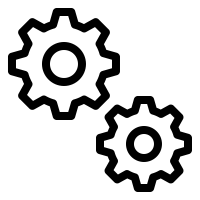
\includegraphics[height=0.6\textheight]{gears.png}

  \begin{columns}[onlytextwidth, T]
  \column{0.4\textwidth}
  \begin{exampleblock}{Avantages}
    \begin{itemize}
    \item Simple
    \item Rapide
    \item Passe à l'échelle
    \end{itemize}
  \end{exampleblock}

  \column{0.4\textwidth}
  \begin{alertblock}{Limitations}
    \textbf{Incomplet}
  \end{alertblock}
  \end{columns}
\end{frame}

\begin{frame}{Le model-checking}

  % 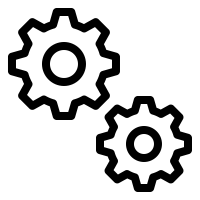
\includegraphics[height=0.6\textheight]{gears.png}

  \begin{columns}[onlytextwidth, T]
  \column{0.4\textwidth}
  \begin{exampleblock}{Avantages}
    \begin{itemize}
    \item Complet
    \item Précis
    \item Modélisation
    \end{itemize}
  \end{exampleblock}

  \column{0.6\textwidth}
  \begin{alertblock}{Limitations}
    \begin{itemize}
    \item Modélisation
    \item Explosion combinatoire
    \item Spécification
    \end{itemize}
  \end{alertblock}
  \end{columns}
\end{frame}

\begin{frame}{Programmation concurrente}

  De plus en plus de systèmes sont concurrents
  \vspace{1em}

  \begin{columns}[onlytextwidth, T]
  \column{0.6\textwidth}
  \begin{alertblock}{Entrelacements}
    \begin{itemize}
    \setlength{\itemsep}{1.5em}
    \item Ordre d'exécution des instructions non-déterministe
    \item Un nombre exponentiel d'entrelacement possible
    \end{itemize}
  \end{alertblock}
  \column{0.4\textwidth}
  \begin{tikzpicture}
    \node at (0, 5.5) {Thread 1};
    \node at (2, 5.5) {Thread 2};
    \draw[->] (0, 5) -- (0, 0);
    \draw[->] (2, 5) -- (2, 0);

    \draw[fill=blue] (-0.2, 4.5) rectangle (0.2, 4.2);
    \draw[fill=blue] (-0.2, 3.5) rectangle (0.2, 2.5);
    \draw[fill=blue] (-0.2, 2) rectangle (0.2, 1.2);

    \draw[fill=red] (1.8, 4.5) rectangle (2.2, 3.5);
    \draw[fill=red] (1.8, 3.2) rectangle (2.2, 3);
    \draw[fill=red] (1.8, 2.8) rectangle (2.2, 2.5);
    \draw[fill=red] (1.8, 2) rectangle (2.2, 0.8);
  \end{tikzpicture}
  \end{columns}
  $\rightarrow$ \alert{plus d'erreurs potentielles}
\end{frame}

\begin{frame}[fragile]{Identifier les variables locales}
\begin{columns}[onlytextwidth, c]
  \column{0.55\textwidth}
  \begin{block}{Problème}
  \begin{itemize}
    \setlength{\itemsep}{1.5em}
    \item Différentes variables de même nom
    \item Même variable dans des contextes différents
  \end{itemize}
  \end{block}

  \vspace{3em}

  $\rightarrow$ Solution partielle\\
    \texttt{main::k}, \texttt{fact::k}

  \column{0.45\textwidth}
\begin{lstlisting}[language=C]
int fact(@\textcolor{red}{int k}@) {
  if (k <= 1)
    return 1;
  else
    return k*@\textcolor{red}{fact(k-1)}@;
}
int main() {
  @\textcolor{red}{int k}@ = fact(3);
  return 0;
}
\end{lstlisting}
\end{columns}
\end{frame}

\begin{frame}[fragile]{Manipuler les positions du code}
\begin{columns}[onlytextwidth, c]
  \column{0.55\textwidth}
  \begin{itemize}
    \setlength{\itemsep}{1.5em}
    \item Utiliser des marqueurs
    \item \alert{Éviter les numéros de ligne}
  \end{itemize}

  \vspace{5em}
  $\rightarrow$ Les labels

  \column{0.45\textwidth}
\begin{lstlisting}
void* bat1(void* d) {
  int i, e = 100;
  for(i=0; i<3; i++) {
    while (e > 0)
        e--;
    // Recharge
    @\textcolor{red}{p1:}@ e = 100;
  }
  pthread_exit(NULL);
}
\end{lstlisting}
\end{columns}
\end{frame}

%% Remplacer par des graphiques ??
\begin{frame}{Résultat expérimentaux}
\begin{table}[tbp]
  \scriptsize
  \centering
\label{tbl:resultats}
\caption{Résultats de la vérification}
\begin{tabular}{|l|l|l|l|}
\hline
Scénario de test           & CBMC                 & ESBMC            & Résulat attendu \\
\hline
answer\_simple             & ERROR MAYBE          & ERROR MAYBE      & ERROR MAYBE     \\
\rowcolor{light-gray}
  answer\_simple\_valid      & \textcolor{red}{\textbf{ERROR MAYBE}} & VALID MAYBE      & VALID MAYBE     \\
battery\_simple            & ERROR SURE           & ERROR SURE       & ERROR SURE      \\
\rowcolor{light-gray}
battery\_var               & ERROR SURE           & \textbf{*}\footnote{Erreur à l'exécution}& ERROR SURE      \\
crossing\_exclusive\_green & VALID MAYBE          & VALID MAYBE      & VALID MAYBE     \\
crossing\_exclusive\_mutex & VALID MAYBE          & VALID MAYBE      & VALID MAYBE     \\
crossing\_GF\_green        & ERROR MAYBE          & ERROR MAYBE      & ERROR MAYBE     \\
crossing\_order            & VALID MAYBE          & VALID MAYBE      & VALID MAYBE     \\
prod\_cons\_mutex          & VALID MAYBE          & VALID MAYBE      & VALID MAYBE     \\
\rowcolor{light-gray}
  prod\_cons\_simple         & ERROR SURE           & \textcolor{red}{\textbf{VALID SURE}} & ERROR SURE      \\
race                       & ERROR MAYBE          & ERROR MAYBE      & ERROR MAYBE     \\
\hline
\end{tabular}
\end{table}
\end{frame}

\begin{frame}{Résultats expérimentaux}
\begin{table}[tbp]
\centering
\scriptsize
\label{tbl:performances}
\caption{Temps d'exécutions}
\begin{tabular}{|l|c|c|c|c|}
\hline
                           & \multicolumn{2}{c|}{CBMC} & \multicolumn{2}{c|}{ESBMC}\\
Scénario de test           & Temps (s) & Mémoire (MB) & Temps (s) & Mémoire (MB) \\
\hline
answer\_simple             & 0.87      & 42           & 5.57      & 56           \\
\rowcolor{light-gray}
answer\_simple\_valid      & 0.81      & 41           & 12.91     & 72           \\
battery\_simple            & 1.07      & 42           & 13.95     & 61           \\
\rowcolor{light-gray}
battery\_var               & 666.04    & 954          & N/A       & OOM          \\
crossing\_exclusive\_green & 2.93      & 44           & 32.12     & 119          \\
crossing\_exclusive\_mutex & 1.73      & 44           & 32.20     & 120          \\
crossing\_GF\_green        & 1.99      & 46           & 41.70     & 117          \\
crossing\_order            & 1.02      & 40           & 11.62     & 56           \\
prod\_cons\_mutex          & 10,046.32 & 593          & 229,99    & 28           \\
\rowcolor{light-gray}
prod\_cons\_simple         & 1.70      & 52           & 454.00    & 2711         \\
race                       & 1.08      & 41           & 5.65      & 28           \\
\hline
\end{tabular}
\end{table}
\end{frame}

\end{document}